
\begin{frame}
    \frametitle{Деревья лиенйных расщеплений (LST)}
	Расщепления по линейным формам над полем $\mathbb{F}_2$
    \begin{columns}
        \begin{column}{3cm}
            Вырожденый лист
            \tikzstyle{end} = [circle, minimum size = 0.1cm, draw, inner sep = 0.1pt]
\tikzstyle{leaf} = [circle, minimum size = 0.6cm, draw, inner sep = 0.1pt, blue]
            
\tikzstyle{level 1}=[level distance = 1cm, sibling distance = 1cm]
\tikzstyle{level 2}=[level distance = 1.5cm, sibling distance = 1.5cm]
\tikzstyle{level 3}=[level distance = 1.5cm, sibling distance = 1.8cm]


    
\begin{tikzpicture}[label distance = 8mm]
	\node [end] (z){}
        child {
        	node[end] (b) {}
            child {
    			node {$\vdots$}
		        edge from parent
	    		node[left] {}
			}
		    child {
		        node[end] {}
                child {
                  	node {\alert{no sol.}}
                    edge from parent
                    node[left] {$y = 0$}
                }
                child {
        			node {$\vdots$}
		           	edge from parent
        		    node[right] {$y = 1$}
		        }
	            edge from parent
		        node[right] {$x + y = 1$}
            }
           	edge from parent
            node[left] {$x = 0$}
        }
        child {
        	node (b) {$\vdots$}
           	edge from parent
            node[right] {}
        };
\end{tikzpicture}

%%% Local Variables: 
%%% mode: latex
%%% TeX-master: t
%%% End: 

        \end{column}
        \begin{column}{3cm}
            Выполняющий набор
            \tikzstyle{end} = [circle, minimum size = 0.1cm, draw, inner sep = 0.1pt]
\tikzstyle{leaf} = [circle, minimum size = 0.6cm, draw, inner sep = 0.1pt, blue]
            
\tikzstyle{level 1}=[level distance = 1cm, sibling distance = 1cm]
\tikzstyle{level 2}=[level distance = 1.5cm, sibling distance = 1.5cm]
\tikzstyle{level 3}=[level distance = 1.5cm, sibling distance = 1.8cm]


    
\begin{tikzpicture}[label distance = 8mm]
	\node [end] (z){}
        child {
        	node[end] (b) {}
            child {
    			node {$\vdots$}
		        edge from parent
	    		node[left] {}
			}
		    child {
		        node[end] {}
                child {
        			node {$\vdots$}
		           	edge from parent
        		    node[left] {$z = 1$}
		        }
                child {
                  	node[blue] {\begin{tabular}{c} $x = 0$ \\ $y = 1$ \\ $z = 0$ \end{tabular}}
                    edge from parent
                    node[right] {$z = 0$}
                }
	            edge from parent
		        node[right] {$x + y = 1$}
            }
           	edge from parent
            node[left] {$x = 0$}
        }
        child {
        	node (b) {$\vdots$}
           	edge from parent
            node[right] {}
        };
\end{tikzpicture}

%%% Local Variables: 
%%% mode: latex
%%% TeX-master: t
%%% End: 

        \end{column}
        \begin{column}{3cm}
            Противоречие с клозом
            \tikzstyle{end} = [circle, minimum size = 0.1cm, draw, inner sep = 0.1pt]
\tikzstyle{leaf} = [circle, minimum size = 0.6cm, draw, inner sep = 0.1pt, blue]
            
\tikzstyle{level 1}=[level distance = 1cm, sibling distance = 1cm]
\tikzstyle{level 2}=[level distance = 1.5cm, sibling distance = 1.5cm]
\tikzstyle{level 3}=[level distance = 1.5cm, sibling distance = 1.8cm]


    
\begin{tikzpicture}[label distance = 8mm]
	\node [end] (z){}
        child {
        	node[end] (b) {}
   		    child {
		        node {\alert{(*)}}
	            edge from parent
		        node[left] {$x + y = 0$}
            }
            child {
    			node {$\vdots$}
		        edge from parent
	    		node[right] {}
			}
           	edge from parent
            node[left] {$x = 0$}
        }
        child {
        	node (b) {$\vdots$}
           	edge from parent
            node[right] {}
        };
\end{tikzpicture}

%%% Local Variables: 
%%% mode: latex
%%% TeX-master: t
%%% End: 

        \end{column}
    \end{columns}
    
	$\Phi$ опровергает $(x_1 \lor x_2 \dots \lor x_k)$ $\Leftrightarrow$ $\Phi \land (x_i = 1)$ невыполнима $\forall i$.
\end{frame}

\begin{frame}
    \frametitle{Splitting trees}
    $(\lnot x \lor y) \land (x \lor \lnot y) \land (\lnot y \lor z) \land
    	(y \lor \lnot z) \land (x \lor z) \land (\lnot x \lor \lnot z)$ 
	\only<1>{\tikzstyle{end} = [circle, minimum size = 0.1cm, draw, inner sep = 0.1pt]
\tikzstyle{leaf} = [circle, minimum size = 0.6cm, draw, inner sep = 0.1pt, blue]
            
\tikzstyle{level 1}=[level distance = 1.5cm, sibling distance = 3cm]
\tikzstyle{level 2}=[sibling distance = 3cm]
\tikzstyle{level 3}=[sibling distance = 3cm]
    
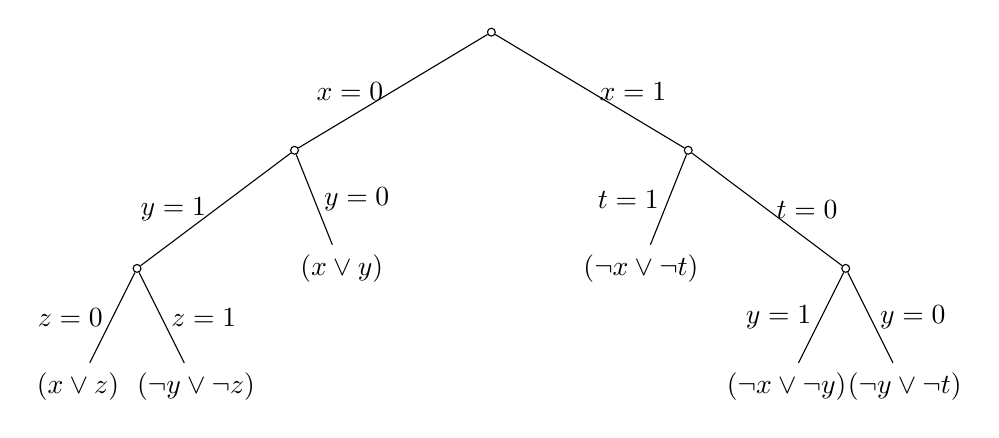
\begin{tikzpicture}[label distance=8mm]
	\node [end] {}
        child {
        	node[end] {}
           	child {
               	node[end] {}
               	child {
                	node {\alert{$(x \lor z)$}}
	                edge from parent
		            node[left] {$z = 0$}
	            }
			    child {
	                node {\alert{$(\neg y \lor \neg z)$}}
	                edge from parent
		            node[right] {$z = 1$}
	            }
                edge from parent
	            node[left] {$y = 1$}
            }
            child[sibling distance = 1.2cm] {
               	node {\alert{$(x \lor y)$}}
                edge from parent
	            node[right] {$y = 0$}
            }
           	edge from parent
            node[left] {$x = 0$}
        }
        child {
        	node[end] {}
            child[sibling distance = 1.2cm] {
            	node {\alert{$(\neg x \lor \neg t)$}}
                edge from parent
                node[left] {$t = 1$}
            }
            child {
            	node[end] {}
                child {
            		node {\alert{$(\neg x \lor \neg y)$}}
	                edge from parent
    	            node[left] {$y = 1$}
        	    }
                child {
            		node {\alert{$(\neg y \lor \neg t)$}}
                	edge from parent
	                node[right] {$y = 0$}
    	        }
                edge from parent
                node[right] {$t = 0$}
            }
           	edge from parent
            node[right] {$x = 1$}
        };
\end{tikzpicture}

%%% Local Variables: 
%%% mode: latex
%%% TeX-master: t
%%% End: 
}
	\only<2>{\tikzstyle{end} = [circle, minimum size = 0.1cm, draw, inner sep = 0.1pt]
\tikzstyle{leaf} = [circle, minimum size = 0.6cm, draw, inner sep = 0.1pt, blue]
            
\tikzstyle{level 1}=[level distance = 1.5cm, sibling distance = 5cm]
\tikzstyle{level 2}=[sibling distance = 4cm]
\tikzstyle{level 3}=[sibling distance = 1.5cm]
    
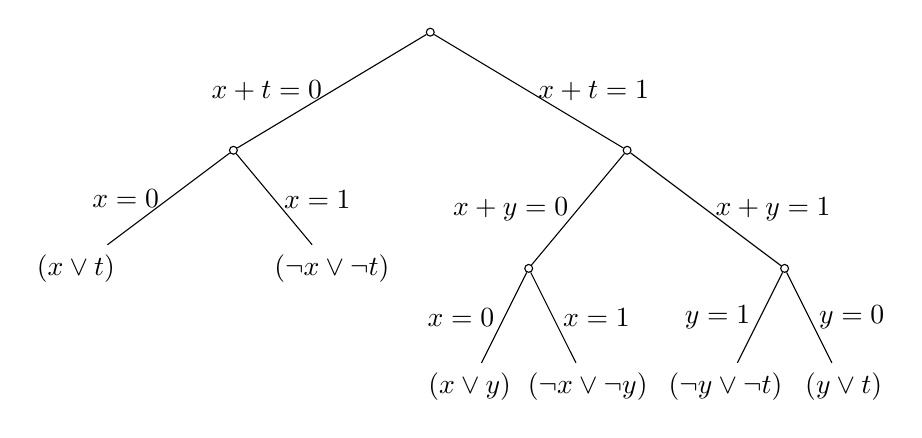
\begin{tikzpicture}[label distance=8mm]
	\node [end] {}
        child {
        	node[end] {}
           	child {
               	node {\alert{$(x \lor t)$}}
                edge from parent
	            node[left] {$x = 0$}
            }
            child[sibling distance = 2.5cm] {
               	node {\alert{$(\neg x \lor \neg t)$}}
                edge from parent
	            node[right] {$x = 1$}
            }
           	edge from parent
            node[left] {$x + t = 0$}
        }
        child {
        	node[end] {}
            child[sibling distance = 2.5cm] {
                node[end] {}
                child {
            		node {\alert{$(x \lor y)$}}
	                edge from parent
    	            node[left] {$x = 0$}
        	    }
                child {
            		node {\alert{$(\neg x  \lor \neg y)$}}
                	edge from parent
	                node[right] {$x = 1$}
    	        }
                edge from parent
                node[left] {$x + y = 0$}
            }
            child {
            	node[end] {}
                child {
            		node {\alert{$(\neg y \lor \neg t)$}}
	                edge from parent
    	            node[left] {$y = 1$}
        	    }
                child {
            		node {\alert{$(y \lor t)$}}
                	edge from parent
	                node[right] {$y = 0$}
    	        }
                edge from parent
                node[right] {$x + y = 1$}
            }
           	edge from parent
            node[right] {$x + t = 1$}
        };
\end{tikzpicture}

%%% Local Variables: 
%%% mode: latex
%%% TeX-master: t
%%% End: 
}
\end{frame}


\begin{frame}
    \frametitle{Алгоритм Сето и Тамаки}

	\begin{itemize}
		\item{} [Seto, Tamaki, 2011] Алгоритм для Formula-SAT над полным бинарным базисом. Для формул размера $cn$ алгоритм
		    работает $2^{(1 - \mu_c)n}$ шагов, где $\mu_c$~--- константа.
        \pause
		\item Алгоритм использует расщепление по линейным комбинациям.
	\end{itemize}    
\end{frame}


\begin{frame}
    \frametitle{Верхние оценки}

    \begin{itemize}
		\item Линейные системы над $\mathbb{F}_2$:
			\begin{itemize}
				\item трудны для резолюций;
				\item просты для LST.
			\end{itemize}
        \pause
		\item Perfect matching principle для графов с нечетным числом вершин:
		    \begin{itemize}
        		\item трудны для резолюций [Разборов, 2003];
				\item просты для LST.
			\end{itemize}
        \pause
		\item Игры с фишками.
			\begin{itemize}
				\item Пусть $\phi$ формула в КНФ обощначим за $\phi^{\oplus}$ КНФ формулу, полученную из $\phi$ путем подстановки
		            $x_1 \oplus x_2$ для каждой переменной $x$. 
				\item{} [Urquhart, 2011] Размер древесного вывода в резолюциях $\phi^{\oplus}$ не менее $2^{d(\phi)}$, где
		            $d(\phi)$ минимальная глубина резолюционного вывода для  $\phi$.
				\item{} [Urquhart, 2011] Для игры с фишками $Peb(G_n)$ выполнено: $d(Peb(G_n)) = \Omega(n / \log(n))$ и $Peb(G_n)$
		            имеет $O(n)$ древесный резолюционный вывод.
				\item Древесный резолюционный вывод для $Peb^\oplus(G_n)$ не менее $2^{n / \log n}$, но $Peb^\oplus(G_n)$ имеет
		            LST размера $O(n)$. 
			\end{itemize}
	\end{itemize}
\end{frame}




\begin{frame}
    \frametitle{Linear systems}

    \begin{columns}
		\begin{column}{1cm}
			Unsatisfiable system:

			$\left\{ \begin{aligned}
				f_1 = \alpha_1 \\
				f_2 = \alpha_2 \\
				\dots\\
				f_m = \alpha_m
			\end{aligned}\right.$
		\end{column}


		\begin{column}{9cm}
			\tikzstyle{end} = [thin, circle, minimum size = 0.1cm, draw, inner sep = 0.1pt]
\tikzstyle{leaf} = [thin, circle, minimum size = 0.6cm, draw, inner sep = 0.1pt, blue]
            
\tikzstyle{level 1}=[level distance = 1.5cm, sibling distance = 1.5cm]
\tikzstyle{level 2}=[level distance = 1.5cm, sibling distance = 4cm]
\tikzstyle{level 3}=[level distance = 2cm, sibling distance = 1.5cm]
\tikzstyle{level 4}=[level distance = 2cm, sibling distance = 1.3cm]

\tikzstyle{edge from parent} = [thin, draw]

    
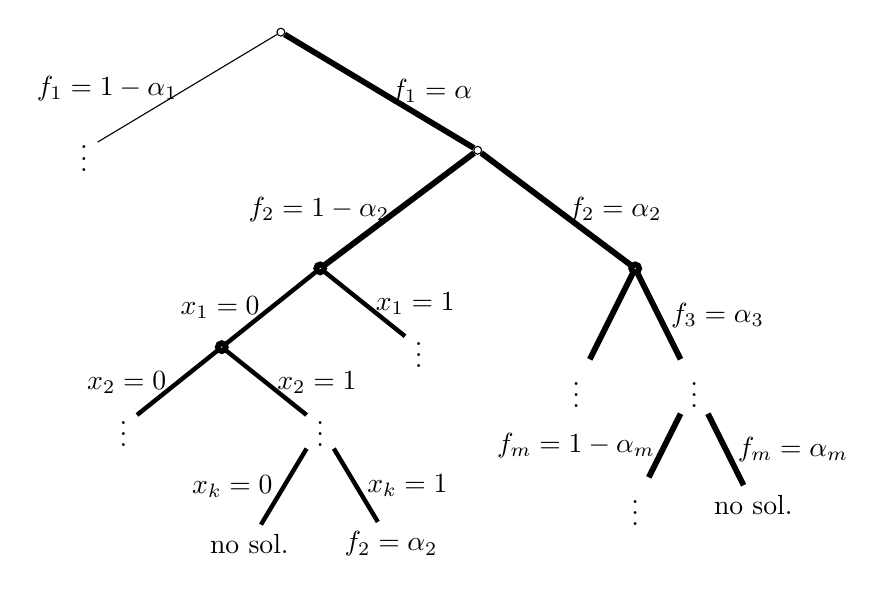
\begin{tikzpicture}[label distance = 8mm]
	\node [end] {}
	    child {
        	node {$\vdots$}
           	edge from parent
            node[left] {$f_1 = 1 - \alpha_1$}
        }
        child {
        	node[end] {}
            child {
		        node[end] {}
                child[level distance = 1.cm, sibling distance = 2.5cm] {
        			node[end] {}
                    child[level distance = 1cm] {
                    	node {$\vdots$}
                    	edge from parent[ultra thick]
	        		    node[left] {$x_2 = 0$}
                    }
                    child[level distance = 1cm] {
                    	node {$\vdots$}
                        child[level distance = 1.5cm, sibling distance = 1.8cm] {
                        	node {\alert{no sol.}}
                            edge from parent[ultra thick]
		        		    node[left] {$x_k = 0$}
                        }
                        child[level distance = 1.5cm, sibling distance = 1.8cm] {
                        	node {\alert{$f_2 = \alpha_2$}}
                            edge from parent[ultra thick]
		        		    node[right] {$x_k = 1$}
                        }
                    	edge from parent[ultra thick]
	        		    node[right] {$x_2 = 1$}
                    }
		           	edge from parent[ultra thick]
        		    node[left] {$x_1 = 0$}
		        }
                child[level distance = 1.cm, sibling distance = 2.5cm] {
                  	node {$\vdots$}
                    edge from parent[ultra thick]
                    node[right] {$x_1 = 1$}
                }
	            edge from parent
		        node[left] {$f_2 = 1 - \alpha_2$}
			}
		    child {
		        node[end] {}
                child {
        			node {$\vdots$}
		           	edge from parent
        		    node[left] {}
		        }
                child {
                  	node {$\vdots$}
                    child{
  		                node {$\vdots$}
			           	edge from parent
        			    node[left] {$f_m = 1 - \alpha_m$}
                    }
                    child{
  		                node {\alert{no sol.}}
			           	edge from parent[line width = 2.1pt]
        			    node[right] {$f_m = \alpha_m$}
                    }
                    edge from parent[line width = 2.1pt]
                    node[right] {$f_3 = \alpha_3$}
                }
	            edge from parent[line width = 2.1pt]
		        node[right] {$f_2 = \alpha_2$}
            }
           	edge from parent[line width = 2.1pt]
            node[right] {$f_1 = \alpha$}
        };
\end{tikzpicture}

%%% Local Variables: 
%%% mode: latex
%%% TeX-master: t
%%% End: 

		\end{column}
	\end{columns}

	$f_2 = x_1 + \dots + x_k$
\end{frame}

\begin{frame}
    \frametitle{Lower bound for 2-fold Tseitin formulas}

    \begin{itemize}
		\item For unsatisfiable $\phi$ a search problem $Search_\phi$: find a
		    falsified clause given a variable assignment.
        \pause 
		\item We prove that it is possible to transform a splitting tree $T$ into a
		    randomized communication protocol for the problem $Search_\phi$ of depth
	        $O(\log |T| \log\log |T|)$ if some variables are known by Alice and other
	        variables are known by Bob.
        \pause
		\item Use a lower bound on the randomized communication complexity of the
		    problem $Search_{TS^2_{G,c}}$ for a 2-fold Tseitin formula $TS^2_{G,c}$
            that follows from [Kalyanasundaram, Schintger 1992] and
            [Beame, Pitassi, Segerlind, 2007].
	\end{itemize}
	\pause
    \begin{theorem}
        In time polynomial in $n$ one may construct a graph $G(V, E)$ on $n$ vertices
        with maximal degree bounded by a constant and a function $c: V \to
        \mathbb{F}_2$ such that the size of any linear splitting tree of
        $TS^2_{(G,c)}$ is at least $\Omega\left(2^{n^{1 / 3} / \log^3(n)} \right)$.
    \end{theorem}
\end{frame}



\begin{frame}
    \frametitle{Res-Lin}

    \begin{itemize}
		\item Literal: $L = x_{1} + x_{2} + \dots + x_{k} = \alpha$,
    		$\lnot L = x_{1} + x_{2} + \dots + x_{k} = \alpha + 1$
		\item Linear clause: $\bigvee_i x_{i, 1} + x_{i, 2} + \dots + x_{i, k_i} =
		    \alpha_i$ or $\lnot \bigwedge x_{i, 1} + x_{i, 2} + \dots + x_{i, k_i} =
            1 + \alpha_i$.
        \pause
		\item Res-Lin:
			\begin{itemize}
				\item Resolution rule: $\frac{(f = 0) \lor D, (f = 1) \lor D'}
            		{D \lor D'}$ 
				\item Weakening rule: $\frac{C}{C'}$ if $C$ semantically implies $C'$
			\end{itemize}
        \pause
		\item \mycolor{blue}{Tree-like} Res-Lin is equivalent to LST.
	\end{itemize}
	\scalebox{0.8}{\tikzstyle{end} = [circle, minimum size = 0.1cm, draw, inner sep = 0.1pt]
\tikzstyle{leaf} = [circle, minimum size = 0.6cm, draw, inner sep = 0.1pt, blue]


\onslide<1->{
	\tikzstyle{level 1}=[level distance = 1.5cm, sibling distance = 6cm, opacity = 0]
	\tikzstyle{level 2}=[sibling distance = 3cm, opacity = 0]
}
\only<3->{
	\tikzstyle{level 1}=[level distance = 1.5cm, sibling distance = 6cm, opacity = 1]
	\tikzstyle{level 2}=[sibling distance = 3cm, opacity = 1]
}






    
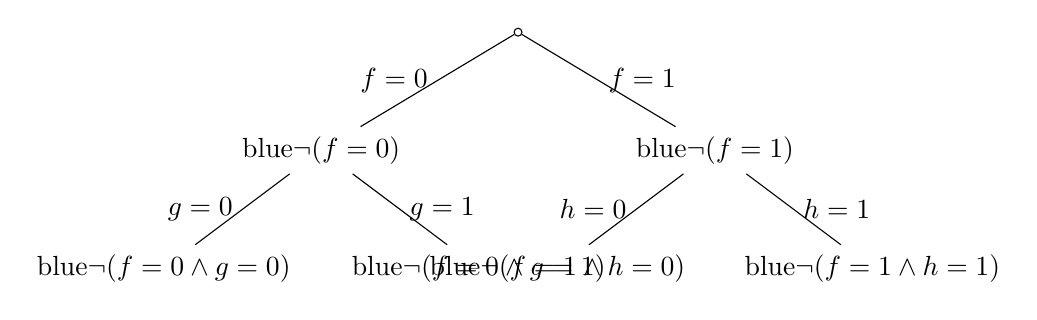
\begin{tikzpicture}[label distance = 8mm, all/.style = {opacity = 0}]
	\node [end] {}
        child {
            node {\mycolor{blue}{$\neg (f = 0)$}}
           	child {
                node {\mycolor{blue}{$\neg (f = 0 \land g = 0)$}}
                edge from parent
	            node[left] {$g = 0$}
            }
            child {
               	node {\mycolor{blue}{$\neg (f = 0 \land g = 1)$}}
                edge from parent
	            node[right] {$g = 1$}
            }
           	edge from parent
            node[left] {$f = 0$}
        }
        child {
            node {\mycolor{blue}{$\neg (f = 1)$}}
           	child {
                node {\mycolor{blue}{$\neg (f = 1 \land h = 0)$}}
                edge from parent
	            node[left] {$h = 0$}
            }
            child {
               	node {\mycolor{blue}{$\neg (f = 1 \land h = 1)$}}
                edge from parent
	            node[right] {$h = 1$}
            }
           	edge from parent
            node[right] {$f = 1$}
        };
\end{tikzpicture}

%%% Local Variables: 
%%% mode: latex
%%% TeX-master: t
%%% End: 
}
\end{frame}



\begin{frame}
    \frametitle{Res-Lin vs Sem-Lin}

    \begin{itemize}
		\item Sem-Lin:
			\begin{itemize}
				\item Semantic rule: $\frac{C_1, C_2}{C'}$ if $C_1 \land C_2$
		            semantically implies $C'$
				\item Weakening rule: $\frac{C}{C'}$ if $C$ semantically implies $C'$
			\end{itemize}
	\end{itemize}

	\pause
    \begin{theorem}
        Res-Lin p-simulates Sem-lin.
    \end{theorem}

	\pause
    \begin{block}{Example}
        How to get $(x + y = 0)$ from $(x = 0)$ and $(y = 0)$ in Res-Lin?
    \end{block}


    \begin{columns}
		\begin{column}{5cm}
            \begin{itemize}
            	\item $\frac{(x = 0)}{(x + y = 0) \lor (y = 1)}$
            \end{itemize}
		\end{column}
		\begin{column}{5cm}
            \begin{itemize}
            	\item $\frac{(x + y = 0) \lor (y = 1),(y = 0)}{(x + y = 0)}$
            \end{itemize}
		\end{column}
	\end{columns}
%	\begin{itemize}
%		\item $\frac{(x = 0)}{(x + y = 0) \lor (y = 1)}$
%		\item $\frac{(x + y = 0) \lor (y = 1),(y = 0)}{(x + y = 0)}$.
%	\end{itemize}

	\pause
    \begin{theorem}
        Res-Lin is implication complete.
    \end{theorem}

	\begin{itemize}
        \pause
		\item The weakening rule may be simulated by a polynomial number of pure
	        syntactic rules.
%		 \begin{itemize}
%			\item The simplification rule: $\frac{D \lor (0 = 1)}{D}$; 
%			\item The syntactic weakening rule: $\frac{D}{D \lor (f = \alpha)}$;
%			\item The addition rule: $\frac{D \lor (f_1 = \alpha_1) \lor
%		        (f_2 = \alpha_2)}{D \lor (f_1 = \alpha_1) \lor
%                (f_1 + f_2 = \alpha_1 + \alpha_2 + 1)}$ 
%		\end{itemize}
	\end{itemize}
\end{frame}



\begin{frame}
    \frametitle{R(lin)}

    R(lin) [Raz, Tsameret, 2007] operates with disjunction of linear equalities with
    \mycolor{blue}{integer} coefficients.
    
	\begin{itemize}
		\item Resolution rule: $\frac{A \lor (F_1 = a_1), B \lor (F_2 = a_2)}
    		{A \lor B \lor (F_1 \pm F_2 = a_1 \pm a_2)}$
		\item Weakening rule: $\frac{A}{A \lor (F = a)}$
		\item Simplification rule: $\frac{B \lor (0 = c)}{B}$, where $c \neq 0$. 
	\end{itemize}

	\pause
    \begin{theorem}
    	R(lin) p-similates Res-Lin.    
    \end{theorem}
    
	\medskip

	\pause
	\begin{columns}
		\begin{column}{5cm}
			$x_1 + x_2 + \dots + x_n \equiv 0 \bmod 2$:
			$\left[\begin{aligned}
            	x_1 + &\dots + x_n = 0\\
                x_1 + &\dots + x_n = 2\\
                &\dots \\
                x_1 + &\dots + x_n = 2 \lceil n / 2 \rceil
            \end{aligned}\right.$ 
		\end{column}
		\begin{column}{5cm}
			$x_1 + x_2 + \dots + x_n \equiv 1 \bmod 2$:
			$\left[\begin{aligned}
                x_1 + &\dots + x_n = 1\\
                x_1 + &\dots + x_n = 3\\
                &\dots \\
                x_1 + &\dots + x_n = 2 \lceil (n - 1) / 2 \rceil + 1
            \end{aligned}\right.$
		\end{column}
	\end{columns}
\end{frame}


\begin{frame}
    \frametitle{Futher research}

    \begin{itemize}
		\item Prove lower bound for dag-like Res-Lin.
		\item What is tree-like Res-Lin complexity of the Perfect Matching Principle
		    for $K_{n - 2, n}$? 
		\item Does tree-like Res-Lin p-simulate dag-like Resolution?
		\item Does PCR p-simulate Res-Lin?
		\item Prove lower bound for splitting by linear combinations on
		    \mycolor{blue}{satisfiable} formulas.
	\end{itemize}
\end{frame}


%%% Local Variables: 
%%% mode: latex
%%% TeX-master: t
%%% End: 
